\documentclass{article}
\usepackage{graphicx} % Required for inserting images
\usepackage{amsmath}
\usepackage{amsfonts}
\usepackage{amssymb}
\usepackage{amsthm}
\usepackage{minted}
\title{Hands-On 6: Algorithm Design A.Y. 2024}

\author{F. Boni \and G. Braccini \and S. Ghosh \and G. Trapani}

\newtheorem*{remark}{Remark}
\newtheorem*{theorem}{Theorem}
\newcommand{\argmax}{\mathop{\mathrm{argmax}}\limits}

\date{29 April 2024}
\begin{document}

\maketitle

\section{Exercise 1}
\textbf{Show how to use matrix computation to compute
the diameter \(D\) exactly (time is \(O(n^\omega \log D)\), where \(n^\omega\) is the
cost of binary matrix multiplication, where \(\omega\) is unknown and currently is
only known that \(2 \leq \omega \leq 2.3728596\)).}

Call \(d(i, j)\) the distance between vertices \(i\) and \(j\).

Since we are using adjacency matrices, we can make use of the following property.
\begin{remark}
	Let \(A\) be the adjacency matrix for a graph \(G\) with an added self-loop for each vertex.

	\noindent The element \(\left(i, j\right)\) in the matrix \(A^n\) gives the number of walks of length \(n\)
	from vertex \(i\) to vertex \(j\); in other terms, the element \(A^n[i, j]\) is different from \(0\)
	if and only if \(d(i, j) \leq n\).
\end{remark}

Calling \(A\) the adjacency matrix for the graph \(G\) with an added self-loop for each vertex,
we can now give the pseudocode of the algorithm we can use to compute the diameter:
\begin{minted}[escapeinside=||,mathescape=true
	numbersep=5pt,
	frame=lines,
	framesep=2mm]{python}
def Diameter(A):
	|$ M_{0} \gets A; $|
	|$ d \gets 0; $|
	while |$ \exists (i, j). \ M_k[i, j] = 0 $|: #we know $k \leq \log D$ from the remark 
		|$ M_{k+1} \gets M_{k}^2; $| #multiplication step takes $n^\omega$
	|$ B \gets M_{k-1}; $|
	|$ d \gets 2^{k-1}; $|
	#Now we need to binary search for the result
	for i in [k-2; 0]:
		|$ C \gets B \times M_i; $|
		if |$ \exists (r, c). \ M_i[r, c] = 0 $|: #we add this term
			|$ B \gets C; $|
			|$ d \gets d + 2^i; $|
	return d;
\end{minted}

\pagebreak
\section*{Exercise 2}
\textbf{Prove that any BFS gives a 2-approximation, that is, the computed value is
\(\geq D/2\), where \(D\) is the graph diameter.}

Let \(G\) be the graph we are performing BFS on and \(V\) the set of its vertices.

For our proof, we make use of the following property of BFS.
\begin{remark}
	Let \(a\) be a vertex in \(G\). Let \(T\) be the breadth-first tree rooted at \(a\).

	\noindent For every vertex \(v\) in \(G\), the length of the shortest path between \(a\) and \(v\)
	in \(G\) is the length of the path from \(a\) to \(v\) in \(T\).
\end{remark}

\begin{proof}
	We pick a vertex \(a\) to start BFS and construct the tree \(T\).

	Now we take the furthest vertex from \(a\) in \(T\) that is
	\[v = \argmax_{x \in V}(d(a, x)) \]

	We know from triangle inequality that
	\[
		\forall (u, w) \in V. \ d(u, w) \leq 2 \times d(a, v)
	\]

	We proved the length of the longest shortest path is between \(d(a, v)\) and \(2 \times d(a, v)\) and this is
	the definition of diameter thus proving our thesis
	\[
		d(a, v) \leq D \leq 2 \times d(a, v) \implies d(a, v) \geq D/2.
	\]
\end{proof}

\pagebreak
\section*{Exercise 3}
\textbf{Consider the 2-sweep algorithm in an unweighted graph. Prove that this algorithm,
which performs quite well in practice, gives an arbitrary lower value with respect to the diameter D
of the following graph:}

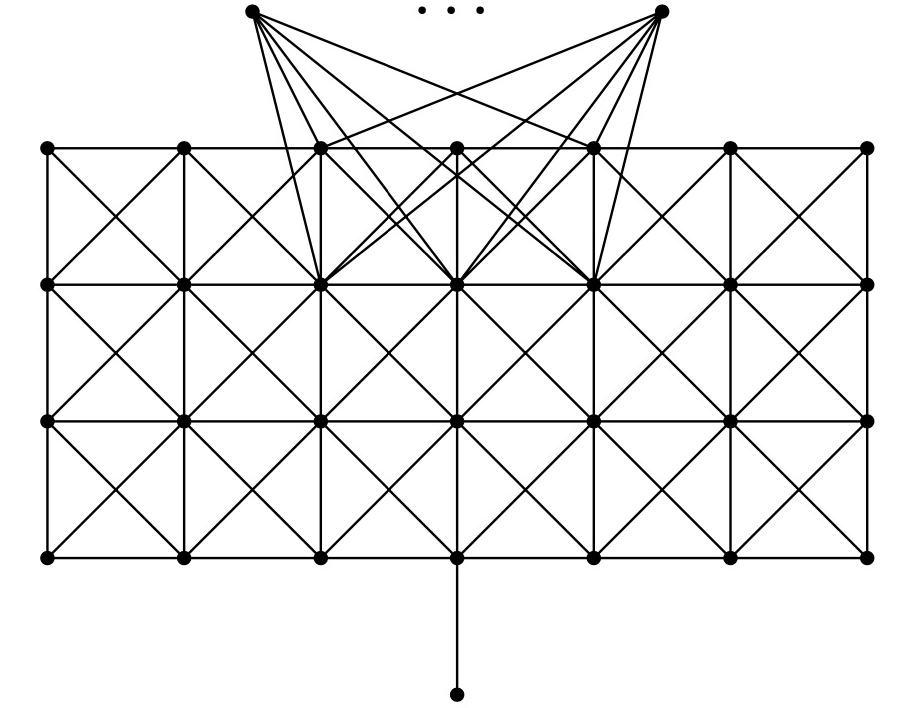
\includegraphics[scale=0.36]{./images/graph.png}

The algorithm is defined as:
\begin{minted}[escapeinside=||,mathescape=true
	numbersep=5pt,
	frame=lines,
	framesep=2mm]{python}
def 2-Sweep(G):
	|$ r \gets $| random node in |$ G $|;
	|$ a \gets $| farthest node from |$ r $|;
	|$ b \gets $| farthest node from |$ a $|;
	return |$ d(a, b) $|;
\end{minted}

First, we consider the graph represented in the picture above.
We can see the diameter is 6, but if we can force the algorithm to choose node \(r\) from the row
above the grid, we get the one on the bottom as \(a\), and the farthest nodes from this \(a\)
are distant 4 which is not the diameter (refer to the picture in the following page).

\pagebreak
\includegraphics*[scale=0.06]{./images/annotated-graph.png}

Now that we have roughly explained our logic, we can generalize.

\begin{theorem}
	Let \(G\) be a graph made up of a grid of \(n \geq 2\) rows, \(2\times n - 1\) columns as in the pictures
	above. If the starting random node \(r\) is chosen from those in the blue rectangle,
	the 2-sweep algorithm returns \(n\).
\end{theorem}

\begin{proof}
	We can prove this by induction on \(k\).
\end{proof}

The number of nodes in the blue rectangle can be chosen such that the probability
of a random node to be chosen in the graph to be in the blue rectangle is arbitrarily high.
Calling \(n\) the number of nodes in the blue rectangle, we can define the probability of choosing
a random node \(r\) among these:
\[
	\begin{aligned}
		& \Pr\left[\text{\(r\) is in the blue rectangle}\right] \\
		&= 1 - \Pr\left[\text{\(r\) is in the grid}\right] \\
		&= 1 - \dfrac{k \times \left(2k - 1\right)}{k \times \left(2k - 1\right) + n}
	\end{aligned}
\]

\qed
\end{document}